 As stated earlier, in order to have a better \gls{snr} one has to integrate more flux. Thus the use of a broader spectrum should improve the performances of the DBC. But as explained in the last section the mathematical formalism doesn't hold in the case of polychromatic light. One has to make the assumption of the input signal being "flat-spectrum" as well as considering the spectral response of the component wavelength independent in order to get it work. The aim of this section is to present the results of a study of the performances of the DBC in the case of polychromatic light. 
 
Using the Beam propagation method to simulate the component behaviour, our simulated polychromatic light is composed of the sum of 50 Diracs of same weight in Fourier's space.  This should be a good
approximation for short bandwidth, less for larger but as those simulations are very time consuming,
the number of diracs wasn't increased to keep the same "density of diracs". Nevertheless no sensible differences were seen in the case of more Dirac. 

The first studied thing is the impact of the V2PM condition number regarding the bandwidth of the input signal. The simulations are performed on the previously optimized component for a "flat spectrum" centred on 3.4 \si{\micro\meter}. Same parameters of convergence, boundary condition and Padé order are used than in the First case. The result of these simulation are shown in Fig.  \ref{fig:cond_nofan}

The integrating area to estimate the phases and visibilities at each outputs is a 1 by 1 micrometer square in the case of the component without fan-out for reasons explained in previous sections. In the case of the component with a fan-out, the area used is the wave-guide cross section,but in this case the V2PM matrix is quite independent of this area (as seen in the previous section).

It appears that for the component without the fan-out, the
condition number oscillate between 5.5 an 7.5 for bandwidth narrower
than 40 nm. It then slowly rises for bandwidth below 150 nm and issues
a sharp increase for higher bandwidth (see Fig.
\ref{fig:cond_nofan}). A similar dependency is found for the component with a fan-out except that the condition number issues a drop around 200 nm bandwidth. Moreover the conditions number from both component are similar at lower bandwidth but are almost 2 times lower at higher bandwidth for the component with a fan-out. This suggest that the component with a fan-out could be more stable at larger bandwidth. Similar dependency has been reported by Saviauk et al. \cite{saviauk} for experimental data on a square array DBC.  

The dependence of the V2PM condition number regarding the bandwidth of the input signal can be interpreted as the degree of validity of the assumption we made in the mathematical formalism. One can notice that for bandwidth lower than approximately 50 to 70 \si{\nano\meter}  the condition number of the V2PM is stable within $\pm 5 \%$ in the case of the component without fan-out. This bandwidth is up to 100 nm in the case of the component with fan-out. 


\begin{figure}[htbp]
  \centering
  \begin{subfigure}{.5\textwidth}
  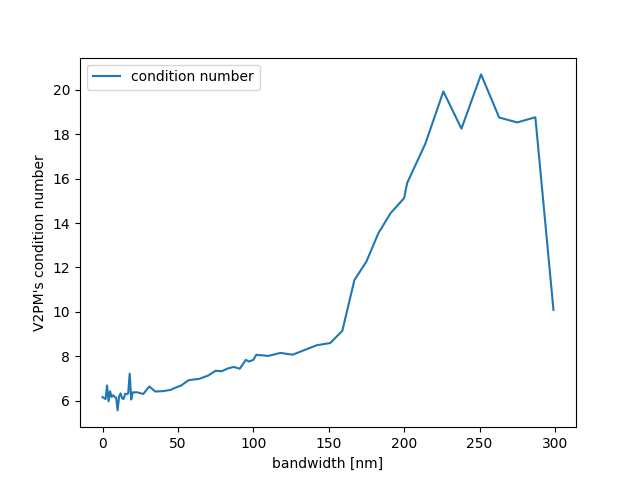
\includegraphics[scale=.5]{picture/cond_BW/cond_nofan.png}
  \caption{For the component without fan-out}
    \end{subfigure}%
  \begin{subfigure}{.5\textwidth}
  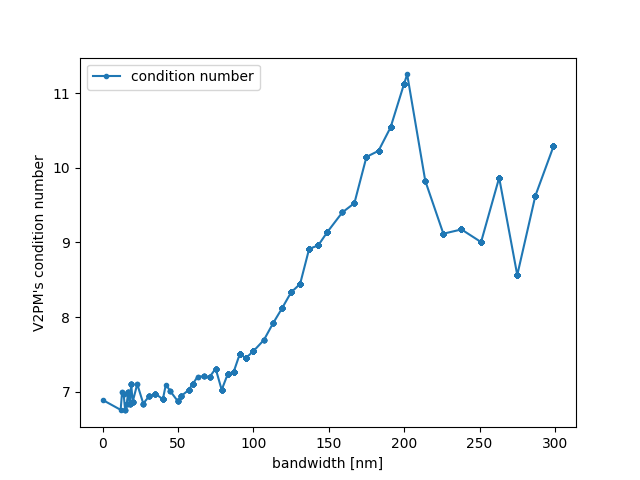
\includegraphics[scale=.5]{picture/cond_BW/cond_fan.png}
  \caption{For the component with a fan-out}
  \end{subfigure}
  \caption{Condition number of the V2PM for different
    bandwidth using the component with and without fan-out. Both DBC part have the same dimensions.}
  \label{fig:cond_nofan}
\end{figure}

However the condition number of the V2PM doesn't give a conclusive statement of the performances of the DBC. Therefore a simulation of the retrieved phase and visibility using the P2VM on simulated data has been performed.
